\subsection{Graph Databases}
A graph database management system (graph database) \citep{robinson13} is an online database management system %with Create, Read, Update, and Delete (CRUD) methods, and is 
based on graph theory. The term graph theory has been used in centuries, and was first introduced by the Swiss mathematician Leonard Euler (1707-1783) when he in 1736 proved that there does not exist a closed walk that crossed exactly once each of the seven bridges of the river Pregel in Köningsberg, now called Kaliningrad\citep{alexanderson06}. Figure \ref{fig:7bridgesEuler} shows Eulers original drawings from his paper written in 1736 \citep{euler1741} of the bridges in Köningsberg. 

\begin{figure}[H]
  \centering
  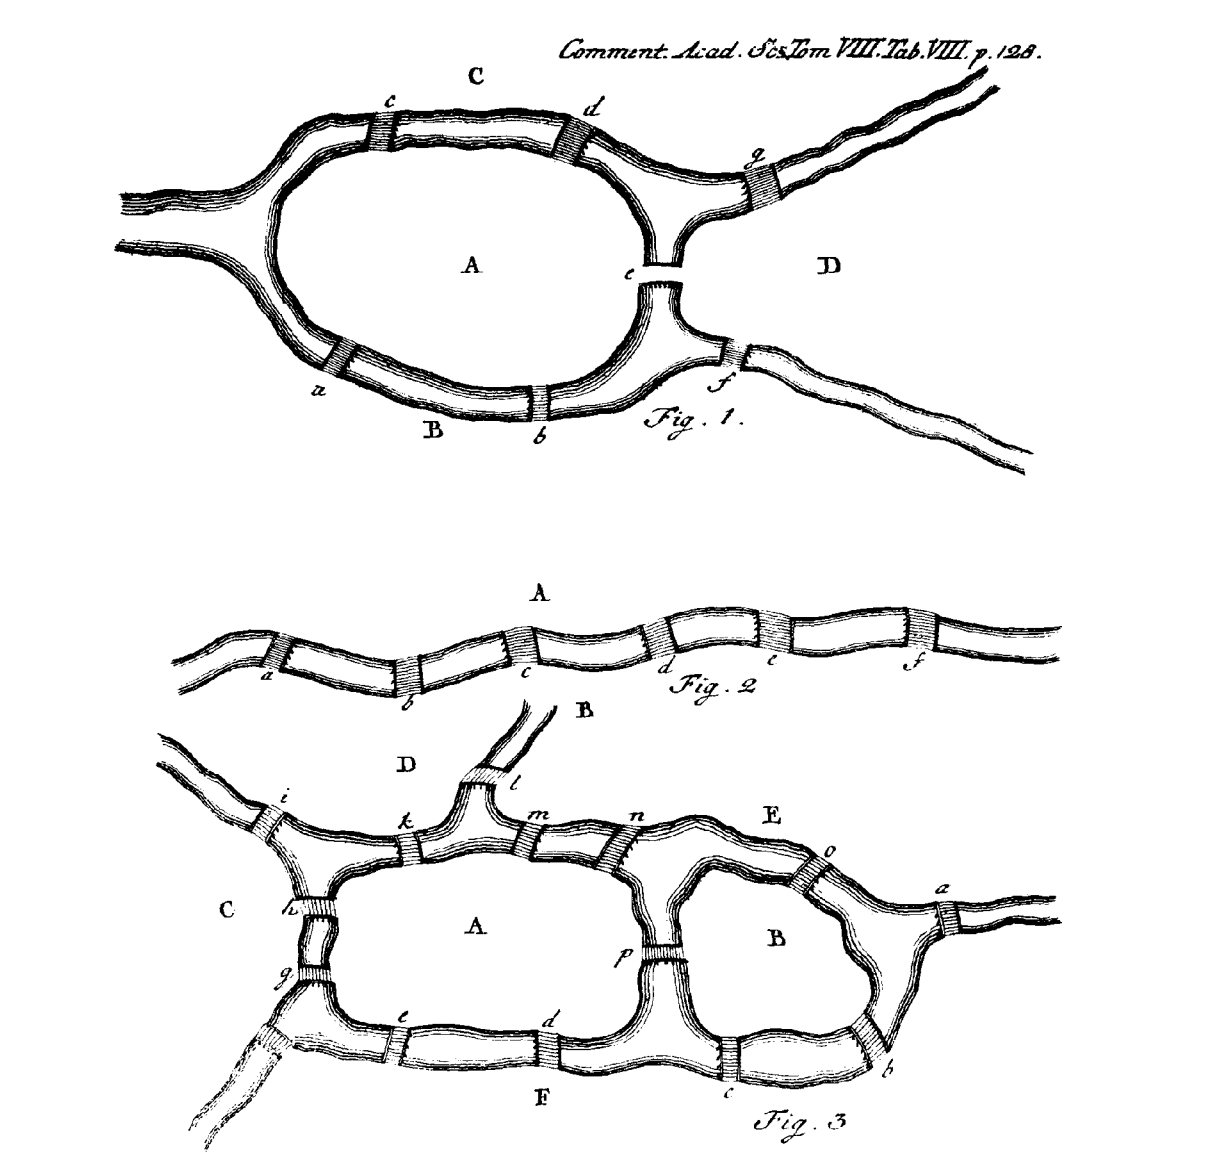
\includegraphics[width=4in]{assets/7bridges-euler.png}
  \caption{\textit{Eulers original drawing of the Seven Bridges of Köningsberg}} 
  \label{fig:7bridgesEuler}
\end{figure}

Based on the solution of the ``Seven Bridges of Köningsberg''-problem, Euler presented a theorem that states that if the graph is planar and connected, and if \textit{v} is the number of vertices, \textit{e} is the number of edges and \textit{f} is the number of faces (regions between edges of a plane graph that does not have any edges in it), then 
\newline
\newline
\centerline{$v-e+f=2$}
\newline
\newline
This means, with respect to the ``Seven Bridges of Köningsberg''-problem, that if it does not exists a path in the graph that lets you visit every node using every edge exactly once, the sum will not be 2. We have illustrated the bridges in Köningsberg as a graph in figure \ref{fig:7bridgesIllustration} and simplified the illustration in figure \ref{fig:7bridgesSimplification}. We see that the graph consists of 4 vertices, 7 edges and 4 faces. The faces are specified with numbers 1-4 in figure \ref{fig:7bridgesSimplification}. If we use the theorem described above we see that $4-7+4\neq2$, which is consistent with Eulers proof from 1736. 

\begin{figure}[H]
  \centering
  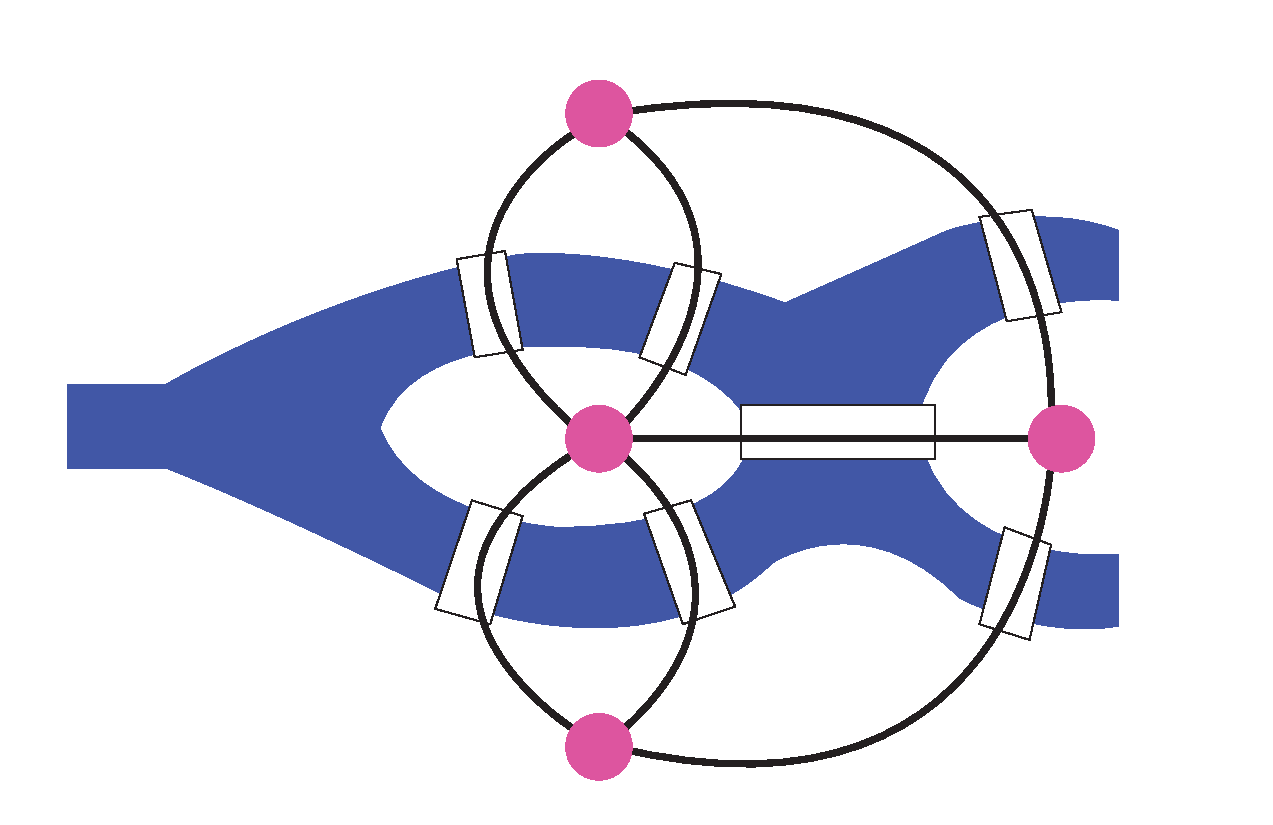
\includegraphics[width=4in]{assets/7bridges.pdf}
  \caption{\textit{Illustration of the Seven Bridges of Köningsberg as a graph}}
  \label{fig:7bridgesIllustration}
\end{figure}

\begin{figure}[H]
  \centering
  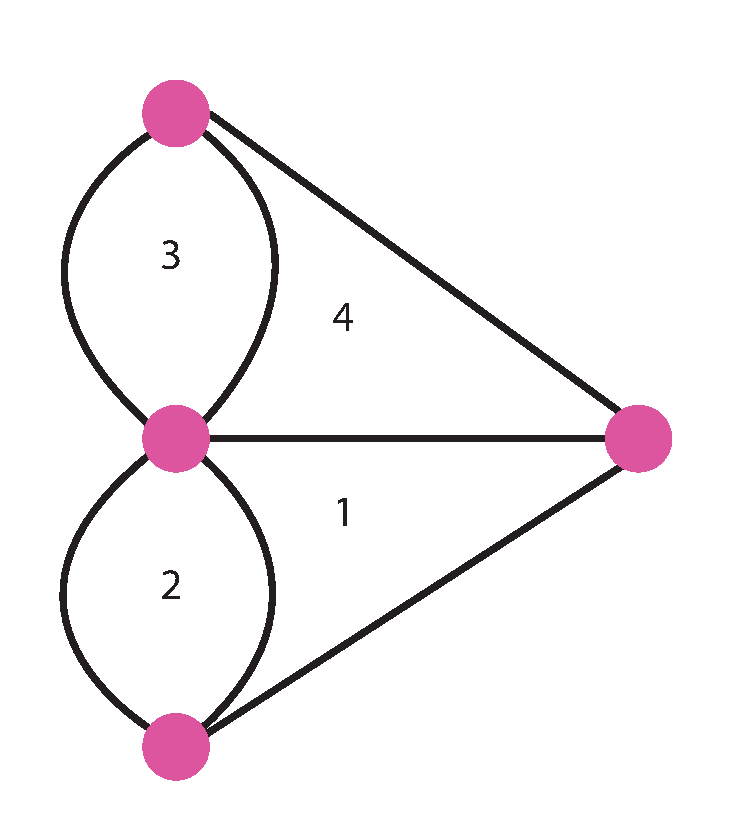
\includegraphics[width=2in]{assets/7bridges2.pdf}
  \caption{\textit{The simplified graph of the Seven Bridges of Köningsberg}} 
  \label{fig:7bridgesSimplification}
\end{figure}

Graph databases uses graph structures for semantic queries with nodes, edges, and properties to represent and store data.
Nodes represent entities, such as people, accounts, or bus stops, properties are relevant information that relate to the nodes and edges, and edges are the lines that connect the nodes and properties, defining the relationship between them. Most of the information is stored in the edges, for instance the travel time or travel demand between to bus stops. 
%Må omformuleres
Applications of graph databases can include calculating routes and finding the shortest path between locations in a network such as a road or rail network, airspace network, or logistical network, finding the center of a region, and calculate the intersection between two or more regions \citep[p.102]{robinson13}. 
%Må omformuleres Compared to relational databases, are graph databases often faster for associative data sets, and map more directly to the structure of object-oriented applications. They can scale more naturally to large data sets as they do not typically require extensive join operations. A drawback to graph databases is the inertia of finding all objects of a specific type.  The following operations are not recommended using graph databases: large, set-oriented wueries, graph global operations and simple, aggregate-oriented queries\citep[p. 40-41]{bruggen14}

\subsubsection{Neo4j}
\label{subsubsec:neo4j}
Neo4j\citep{website:neo4j} is an open-source graph database, implemented in Java, and is ranked the most popular graph database \citep{website:graphdbranking}. It is a native graph database optimized and designed for storing and managing graphs, and is known for extremely fast traversals of relationship. The underlying data model of Neo4j is the labeled property graph, and is one of the most generic and versatile of all graph models\citep[p.73]{robinson13}. This graph data model gives four different fundamental building blocks to structure and store data, including nodes to store entity information, relationships to connect nodes to another, properties for relevant information, and labels for creating subgraphs. 

A query that is extremely well suited for graph databases are queries for finding the paths between different nodes on your graph, and Neo4j can be used to see whether a path exist, finding the optimal path, and looking for variability of the path\citep[p. 51]{bruggen14}. Neo4j includes built-methods for finding the shortest path, including:

\begin{itemize}
\item Dijkstra's algorithm\citep{cormen09}, which is one of the best-known algorithms to calculate the shortest weighted path between two points in a graph, using the properties of the edges as a weight or costs of that link.
\item A* search\citep{russel10}, which is a variation of Dijkstra's original ideas, but uses heuristics to predict more efficiently the shortest path exploration. A* search explores potential graph paths by it calculates the past path cost and the future path cost of the different options that are possible during the route exploration. 
\end{itemize}

%Sweet spot use cases of neo4j: complex, join-intensive queries, path finding queries\citep[p. 51]{bruggen14}. 

%TODO skrive mer her

%Advantages:
%\begin{itemize} 
%\item Flexibility: model, develop and visualize the world as you experience it. Its simply nodes and relationships. 
%\item Performance: Hyper-connectivity at speed. 
%\item Scalability: Scales up and out, supporting tens of billions of nodes and relationships, and hundred of thousands of ACID transactions per seconds. 
%\item Speed: Able to search trough millions of connections per second, with real time queries that stay fast even as your database grows. 
%\end{itemize}

%\begin{itemize}
%\item Native graph database. 
%\item Property graph. 
%\item Made for real time queries. 
%\item Really fast traversals of relations.
%\item Neo4J has an API that supports traversing - finding shortest path - can weight edges, nodes -
%\end{itemize}
%//en korteste vei mellom n og m men max lengde 3
%match p = shortestPath ( (n) - [*...3]--(m)) return p
%(Vekte kanter: Neo44J har et API som støtter traversering, Dijkstras er innebyd ++ som lar deg vekte kanter - hva er raskeste vei ++)

%Neo4J can be used to evaluate routes after the ants have created route sets.